\documentclass[$fontsize$, width=$width$, height=$height$]{beamer}
\usetheme{Boadilla}

$if(pdflatex)$
  \usepackage[protrusion=true,expansion=true]{microtype}
$endif$

\usepackage{booktabs}
\usepackage{longtable}
\usepackage{multirow}

$if(amsthm)$
  \usepackage{amsthm}
$endif$

$if(customfonts)$
  \let\digamma\relax  
  \usepackage{lucimatx}
$else$
  \usepackage{amsmath}
  \usepackage{amssymb}
$endif$

\usepackage{tikz}
\usepackage[framemethod=tikz]{mdframed}

% texlive 2020
$if(csl-refs)$
\newlength{\cslhangindent}
\setlength{\cslhangindent}{1.5em}
\newenvironment{CSLReferences}[2]
  {$if(csl-hanging-indent)$\setlength{\parindent}{0pt}
  \everypar{\setlength{\hangindent}{\cslhangindent}}\ignorespaces$endif$}
  {\par}
$endif$

$if(creativecommons)$
\usepackage{hyperxmp}
\usepackage[type={CC}, modifier={$creativecommons$}, version={4.0}]{doclicense}
$endif$

\makeindex

\providecommand{\tightlist}{\setlength{\itemsep}{0pt}\setlength{\parskip}{0pt}}

% To pass between YAML and LaTeX the dollar signs are added by CII
% Syntax highlighting #22
$if(highlighting-macros)$
  $highlighting-macros$
$endif$

\author{$author$}
\title{$title$}
\subtitle{$subtitle$}
\date{$date$}

\makeindex

\pretocmd{\tableofcontents}{\begin{minipage}{\textwidth}}{}{}
\apptocmd{\tableofcontents}{\end{minipage}}{}{}

% remove navigation symbols
\setbeamertemplate{navigation symbols}{}

% put titles and links in UofT blue
\definecolor{myblue}{RGB}{0,42,92}
\setbeamercolor{frametitle}{fg=myblue}
\hypersetup{colorlinks,linkcolor=myblue,urlcolor=myblue}

% remove footer
% \setbeamertemplate{footline}{}

% add new footer in myblue with UofT logo
\setbeamercolor{box}{bg=myblue}
\setbeamertemplate{footline}{%
  \begin{beamercolorbox}[wd=\paperwidth,ht=7.5ex,left]{box}
    
\includegraphics[height=7.5ex]{../tex/uoftlogowhite.png}
    % \hspace{0.05\paperwidth}
    % \insertshortauthor
    % \hspace{0.05\paperwidth}
    % \insertshorttitle
    % \hspace{0.05\paperwidth}
    % \insertshortdate
    % \hspace{0.05\paperwidth}
    % \insertframenumber{} / \inserttotalframenumber
  \end{beamercolorbox}
}

% titles in bold
\setbeamerfont{frametitle}{series=\bfseries}

% redefine ball to plain color
% \useinnertheme{circles}

% set enumeration color to myblue
\setbeamercolor{itemize item}{fg=myblue}
\setbeamercolor{itemize subitem}{fg=myblue}
\setbeamercolor{itemize subsubitem}{fg=myblue}

% plain enumeration
\setbeamertemplate{itemize items}[default]
\setbeamertemplate{enumerate items}[default]

% use plain enumeration in TOC
\setbeamertemplate{section in toc}[default]
\setbeamertemplate{subsection in toc}[default]

% custom title page

% Make a custom block
\newenvironment<>{customBlock}[1]{
  \begin{actionenv}#2
    \def\insertblocktitle{#1}
    \par
    \mode<presentation>{
      \setbeamercolor{block title}{fg=white,bg=orange!20!black}
      \setbeamercolor{block body}{fg=black,bg=olive!50}
      \setbeamercolor{itemize item}{fg=orange!20!black}
      \setbeamertemplate{itemize item}[triangle]
    }
  \usebeamertemplate{block begin}
}
{\par\usebeamertemplate{block end}\end{actionenv}}

\begin{document}

% My fancy title page, using transparent text box from mdframe, and icons from fontawesome
{ 
  \hoffset=-12pt
  \begin{frame}[plain,t] 

    \vspace{2em}

    \begin{tikzpicture}
      \node[text width=\paperwidth, fill=white] at (0,0) {
        \begin{tabular}{l}
          \begin{minipage}{\textwidth}
            \vspace{3em}
            {\huge \color{myblue}{\inserttitle}}
            % if subtitle is not empty, add it
            $if(subtitle)$
              \vspace{1em}
              {\newline\Large \color{myblue}{\insertsubtitle}}
            $endif$
          \end{minipage}
        \end{tabular}
      };
    \end{tikzpicture}
    
    % ifelse subtitle is empty, add some space
    $if(subtitle)$
      \vspace{1em}
    $else$
      \vspace{3em}
    $endif$

    \begin{tikzpicture}
      \node[text width=\paperwidth, fill=myblue] at (0,0) {
        % table with text on left and image on the right
        \begin{tabular}{lr}
          % two lines of text as multirow
          \begin{minipage}{.7\textwidth}
            \begin{flushleft}
              {\Large \color{white}{\insertauthor}}\\
              $if(department)$
              \vspace{0.2em}
              {\Large \color{white}{$department$}}\\
              $endif$
              \vspace{1em}
              {\Large \color{white}{\insertdate}} 
            \end{flushleft}
          \end{minipage}
            &
          \begin{minipage}{.3\textwidth}
            \begin{flushright}
              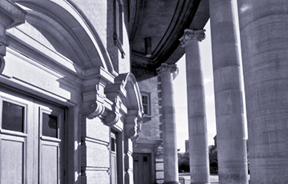
\includegraphics[width=0.3\paperwidth]{../tex/uofthall.png}
            \end{flushright}
          \end{minipage}
        \end{tabular}
      };
    \end{tikzpicture}

    % ifelse subtitle is empty, add some space
    $if(subtitle)$
      \vspace{1em}
    $else$
      \vspace{2em}
    $endif$

    \begin{tikzpicture}
      \node[text width=\paperwidth, fill=white] at (0,0) {
        \begin{tabular}{l}
          
\includegraphics[width=0.2\paperwidth]{../tex/uoftlogoblue.png}
        \end{tabular}
      };
    \end{tikzpicture}   

  \end{frame}
}

% restore hoffset
\hoffset=0pt

% Title page frame
% \begin{frame}
%   \titlepage
% \end{frame}

$if(creativecommons)$
\begin{frame}
  \doclicenseThis
\end{frame}
$endif$

$if(outline)$
\begin{frame}{Outline}
\tableofcontents
\end{frame}
$endif$

$body$

\end{document}
